\documentclass[a4paper]{article}
\usepackage[14pt]{extsizes} 
\usepackage[T2A]{fontenc}
\usepackage[utf8]{inputenc}
\usepackage{natbib}
\usepackage{graphicx}
\usepackage{amsmath}
\usepackage[english, russian]{babel}
\usepackage{fontspec}
\usepackage{amsmath,amsfonts,amssymb,amsthm,mathtools,mathrsfs}
\usepackage{icomma}
\usepackage{fullpage}
\usepackage{ulem}
\usepackage{eufrak}
\usepackage{setspace}
\usepackage{listings}
\usepackage{indentfirst}
\usepackage[left=2cm,right=1.5cm,top=2cm,bottom=2cm]{geometry}
\usepackage{xcolor}
\usepackage{float}
\usepackage{csquotes}

\setmainfont[Ligatures={TeX,Historic}]{Times New Roman}
\setlength{\parindent}{5ex}
\setlength{\parskip}{1em}
\renewcommand{\baselinestretch}{1}

\graphicspath{{images/}}

\definecolor{buzzlightyear}{HTML}{8757A5}
\definecolor{grass}{HTML}{738D06}
\definecolor{literal}{HTML}{F18A2B}
\definecolor{commentcolor}{HTML}{8E908B}

\lstdefinestyle{habrstyle}{
    backgroundcolor=\color{white},   
    commentstyle=\color{commentcolor},
    keywordstyle=\bfseries\color{buzzlightyear},
    numberstyle=\tiny\color{commentcolor},
    stringstyle=\color{grass},
    basicstyle=\ttfamily\footnotesize,
    breakatwhitespace=false,         
    breaklines=true,                 
    captionpos=b,                    
    keepspaces=true,                 
    numbers=left,                    
    numbersep=5pt,                  
    showspaces=false,                
    showstringspaces=false,
    showtabs=false,                  
    tabsize=4
}

\lstset{style=habrstyle}

\begin{document}
    % НАЧАЛО ТИТУЛЬНОГО ЛИСТА
    \begin{center}
        \begin{center}
        \hfill \break
        \normalsize{Санкт-Петербургский государственный политехнический}\\
        \normalsize{университет Петра Великого}\\
        \hfill \break
        \normalsize{\textbf{Высшая школа интеллектуальных систем и}}\\ 
        \normalsize{\textbf{суперкомпьютерных технологий}}\\ 
        \hfill \break
        \hfill \break
        \hfill \break
        \normalsize{Лабораторная работа}\\
        \hfill \break
        \hfill \break
        \normalsize{\LARGE Апериодические сигналы}\\
        \end{center}
        \hfill \break
        \hfill \break
        \hfill \break
        \hfill \break
        \hfill \break
        \hfill \break
        \hfill \break
        \hfill \break
        \hfill \break
        \hfill \break
        \begin{flushright}
            \normalsize{Работу выполнил студент}\\
            \normalsize{3-го курса, группа 3530901/80201}\\
            \normalsize{Солянкин Илья Андреевич}\\
            \hfill \break
            \normalsize{Преподаватель:}\\
            \normalsize{Богач Наталья Владимировна}\\
        \end{flushright}
        \hfill \break
        \hfill \break
        \hfill \break
        \hfill \break
        \begin{center} Санкт-Петербург 2021 \end{center}
        \thispagestyle{empty}
    \end{center}
    % КОНЕЦ ТИТУЛЬНОГО ЛИСТА
    
    % ОГЛАВЛЕНИЕ
    \newpage
        \tableofcontents
    
    % СПИСОК ИЛЛЮСТРАЦИЙ
    \newpage
         \listoffigures
    
    % СПИСОК ЛИСТИНГОВ     
    \newpage
         \lstlistoflistings   
     
    \newpage
        \section{Часть №1: Запуск примеров из \texttt{chap03.ipynb}}
            В первом пункте третьей лабораторной работы нам необходимо запустить все файлы из \texttt{chap03.ipynb}, а также в примере с утечной заменить окно Хэмминга одним из окон, представляемых \texttt{NumPy}.
            Начнем с запуска всех программ.
            
            \begin{figure}[h]
                \centering
                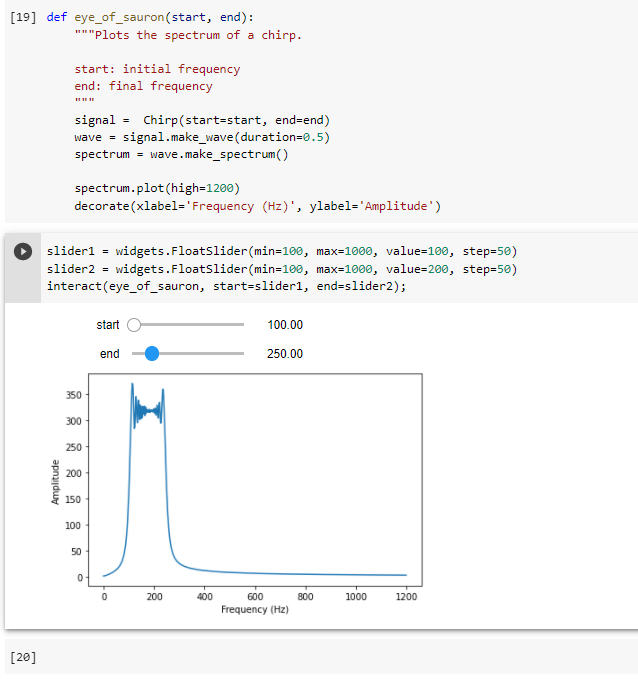
\includegraphics[width=\textwidth]{ex_1_all_working.png}
                \caption{Проверка, что все работает}
                \label{fig:ex_1_all_working}
            \end{figure}
            
            Теперь перейдем к написанию разных окон в примерах с утечкой. Начем с окна Бартлетта:
            
\begin{lstlisting}[language=Python, caption= Окно Бартлетта]
    wave = signal.make_wave(duration)
    wave.window(np.bartlett(len(wave)))
    spectrum = wave.make_spectrum()
    spectrum.plot(high=880)
    decorate(xlabel='Frequency (Hz)')
\end{lstlisting}               
            
            \begin{figure}[H]
                \centering
                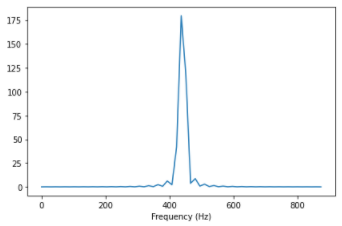
\includegraphics{ex_1_bartlett.png}
                \caption{Замена на окно Бартлетта}
                \label{fig:ex_1_bartlett}
            \end{figure}
            
            После этого напишем окно \texttt{blackman}:
            
\begin{lstlisting}[language=Python, caption= Окно \texttt{blackman}]
    wave = signal.make_wave(duration)
    wave.window(np.blackman(len(wave)))
    spectrum = wave.make_spectrum()
    spectrum.plot(high=880)
    decorate(xlabel ='Frequency (Hz)')
\end{lstlisting}               
            
            \begin{figure}[H]
                \centering
                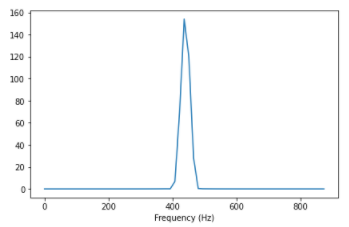
\includegraphics{ex_1_blackman.png}
                \caption{Замена на окно \texttt{blackman}}
                \label{fig:ex_1_blackman}
            \end{figure}
            
            Теперь напишем окно \texttt{hanning}:
            
\begin{lstlisting}[language=Python, caption= Окно \texttt{hanning}]
    wave = signal.make_wave(duration)
    wave.window(np.hanning(len(wave)))
    spectrum = wave.make_spectrum()
    spectrum.plot(high =880)
    decorate(xlabel ='Frequency (Hz)')
\end{lstlisting}               
            
            \begin{figure}[H]
                \centering
                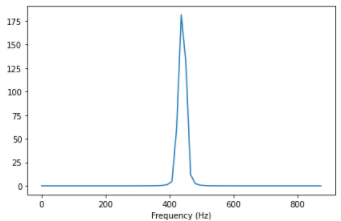
\includegraphics{ex_1_hanning.png}
                \caption{Замена на окно \texttt{hanning}}
                \label{fig:ex_1_blackman}
            \end{figure}
            
            И, наконец, напишем окно \texttt{kaiser}
            
\begin{lstlisting}[language=Python, caption= Окно \texttt{kaiser}]
    wave = signal.make_wave(duration)
    wave.window(np.hanning(len(wave)))
    spectrum = wave.make_spectrum()
    spectrum.plot(high =880)
    decorate(xlabel ='Frequency (Hz)')
\end{lstlisting}               
            
            \begin{figure}[H]
                \centering
                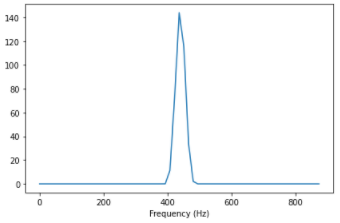
\includegraphics{ex_1_kraiser.png}
                \caption{Замена на окно \texttt{kaiser}}
                \label{fig:ex_1_kraiser}
            \end{figure}
            
            Для болшей наглядности совмстим все графики в одном:
            
\begin{lstlisting}[language=Python, caption= Совмещение всех графиков]
    wave = signal.make_wave(duration)
    wave.window(np.bartlett(len(wave)))
    spectrum = wave.make_spectrum()
    spectrum.plot(high=880)
    decorate(xlabel='Frequency (Hz)')
    
    wave = signal.make_wave(duration)
    wave.window(np.kaiser(len(wave), 10))
    spectrum = wave.make_spectrum()
    spectrum.plot(high =880, color ='green')
    decorate(xlabel ='Frequency (Hz)')
    
    wave = signal.make_wave(duration)
    wave.window(np.hanning(len(wave)))
    spectrum = wave.make_spectrum()
    spectrum.plot(high =880, color ='orange')
    decorate(xlabel ='Frequency (Hz)')
    
    wave = signal.make_wave(duration)
    wave.window(np.blackman(len(wave)))
    spectrum = wave.make_spectrum()
    spectrum.plot( high=880, color ='black')
    decorate(xlabel ='Frequency (Hz)')
\end{lstlisting}               
            
            \begin{figure}[H]
                \centering
                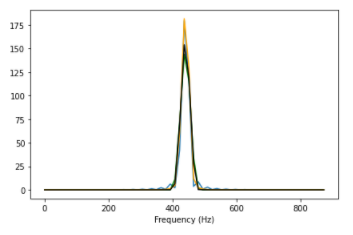
\includegraphics{ex_1_all_in_one.png}
                \caption{Совмещение всех графиков}
                \label{fig:ex_1_all_in_one}
            \end{figure}
    
    \newpage
        \section{Часть №2: Создание \texttt{SawtoothChirp}}
            Во втором пункте третьей лабораторной работы нам необходимо создать класс \texttt{SawtoothChirp}, который бы расширял \texttt{Chirp} и переопределял \texttt{evaluate} для генерации пилообразного сигнала с линейно увеличивающейся частотой.
            
            Для начала имортируем все необходимые нам для выполнения библиотеки:
            
\begin{lstlisting}[language=Python, caption= Импорт библиотек]
    from thinkdsp import Signal, Sinusoid, SquareSignal, TriangleSignal, SawtoothSignal, ParabolicSignal
    from thinkdsp import normalize, unbias, PI2, decorate
    from thinkdsp import Chirp
    import numpy as np
\end{lstlisting}        
            
            После чего напишем сам класс:
            
\begin{lstlisting}[language=Python, caption= Класс \texttt{SawtoothChirp}]
    class MySawtoothChirp(Chirp):
    def evaluate(self, ts):
        freqs = np.linspace(self.start, self.end, len(ts) - 1)
        
        dts = np.diff(ts)
        dphis = PI2 * freqs * dts
        
        phases = np.cumsum(dphis)
        
        
        cycles = phases / PI2
        frac, _ = np.modf(cycles)

        ys = normalize(unbias(frac), self.amp)
        return ys
\end{lstlisting}      
            
            Теперь выведем начальный сегмент полученного сигнала:
            
\begin{lstlisting}[language=Python, caption= Получение начального сегмента]
    signal = MySawtoothChirp(start=220, end=440)
    wave = signal.make_wave(duration=1, framerate=4025)
    wave.segment(start=0, duration=0.02).plot() 
    decorate(xlabel='Time (s)')
\end{lstlisting}               
            
            \begin{figure}[H]
                \centering
                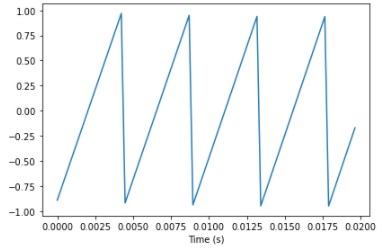
\includegraphics{ex_2_segment_begin.png}
                \caption{Начальный сегмент}
                \label{fig:ex_2_segment_begin}
            \end{figure}
            
            После чего переведм изначальный сигнал в аудио:
            
            \begin{figure}[H]
                \centering
                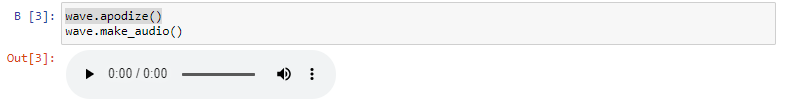
\includegraphics[width=\textwidth]{ex_2_wave_audio.png}
                \caption{Сегмент в аудио}
                \label{fig:ex_2_wave_audio}
            \end{figure}
            
            Затем выведем конечный участок сегмента:
            
\begin{lstlisting}[language=Python, caption= Получение конечного сегмента]
    wave.segment(start=1-0.02, duration=0.02).plot()
    decorate(xlabel='Time (s)')
\end{lstlisting}               
            
            \begin{figure}[H]
                \centering
                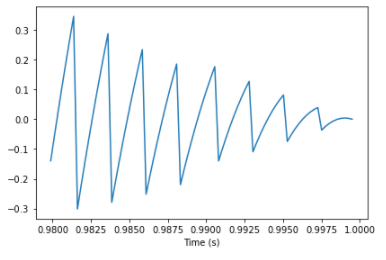
\includegraphics{ex_2_segment_end.png}
                \caption{Конечный сегмент}
                \label{fig:ex_2_segment_end}
            \end{figure}
            
            Наконец, выведем на экран спектрограмму для нашего сигнала:
            
\begin{lstlisting}[language=Python, caption= Спектограмма сигнала]
    sp = wave.make_spectrogram(256)
    sp.plot()
    decorate(xlabel='Time (s)', ylabel='Frequency (Hz)')
\end{lstlisting}               
            
            \begin{figure}[H]
                \centering
                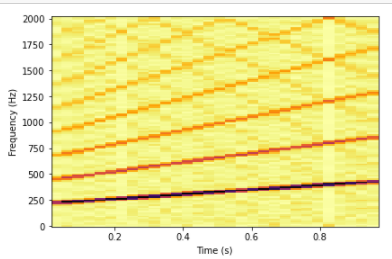
\includegraphics{ex_2_spectogramma.png}
                \caption{Спектограмма сигнала}
                \label{fig:ex_2_spectogramma}
            \end{figure}
            
    \newpage
        \section{Часть №3: Создание меняющегося пилообразного сигнала}
            В третьей части третьей лабораторной работы там необходимо создать пилообразный чирп, меняющийся от 2500 до 3000 Гц и на его основе сгенерировать сигнал длительность. 1с и частотой кадорв в 20кГц. Нарисовать \texttt{Spectrum}.
            
            Для начала создадим сигнал согласно заданию:
            
\begin{lstlisting}[language=Python, caption= Создаие согласо задания сигнала]
    signal = MySawtoothChirp(start=2500, end=3000)
    wave = signal.make_wave(duration=1, framerate=20_000)
\end{lstlisting}    
            
            После этого посмотрим на сегмент этого сигнала:
            
\begin{lstlisting}[language=Python, caption= Сегмент сигнала]
    wave.segment(start=0.9, duration=0.02).plot()
    decorate(xlabel='Time')
\end{lstlisting}               
            
            \begin{figure}[H]
                \centering
                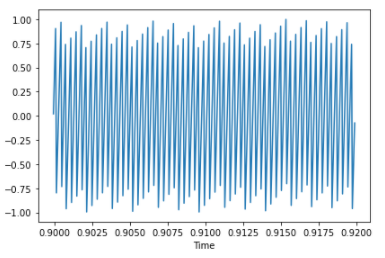
\includegraphics{ex_3_segment.png}
                \caption{Сегмент сигнала}
                \label{fig:ex_3_segment}
            \end{figure}
            
            Затем представим сигнал в виде аудио:
            
            \begin{figure}[H]
                \centering
                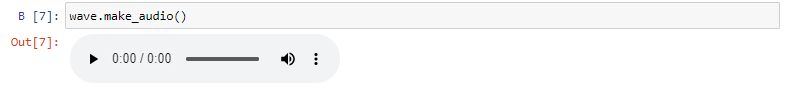
\includegraphics[width=\textwidth]{ex_3_wave_audio.png}
                \caption{Сигнал в аудио}
                \label{fig:ex_3_wave_audio}
            \end{figure}
            
            И, наконец, построим и выведем на экран спект нашего сигнала:
            
\begin{lstlisting}[language=Python, caption= Спектр сигнала]
    spectrum = wave.make_spectrum()
    spectrum.plot()
    decorate(xlabel='Frequency')
\end{lstlisting}               
            
            \begin{figure}[H]
                \centering
                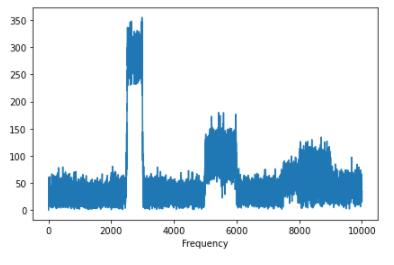
\includegraphics{ex_3_wave_spectr.png}
                \caption{Спектр сигнала}
                \label{fig:ex_3_wave_spectr}
            \end{figure}
            
            В заключение можно сказать, что полученный сигнал очень сильно режет слух, а проанализировав спектр можно сделать вывод, что он содержит большое количество частотных компонент.
            
    \newpage
        \section{Часть №4: Глиссандро}
            В четвертом пунтке третьей лабораторной работы нам необходимо сначала скачать звук глиссандо и распечатать спектограмму первых секунд.
            
            В качестве аудиодорожки я выбрал «Rhapsody in Blue» (George Gershwin), как посоветовали в ThinkDSP.
            
\begin{lstlisting}[language=Python, caption= Получение сегмена из аудиофайла]
    from thinkdsp import read_wave

    wave = read_wave('rhapblue11924.wav')
    segment = wave.segment(start=1.35, duration=1.8-1.35)
    segment.plot()
\end{lstlisting}   
            
             \begin{figure}[H]
                \centering
                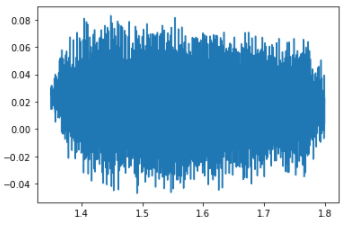
\includegraphics{ex_4_segment.png}
                \caption{Полученный сегмент}
                \label{fig:ex_4_segment}
            \end{figure}
            
            Затем для проверки выведем наш файл в аудио:
            
            \begin{figure}[H]
                \centering
                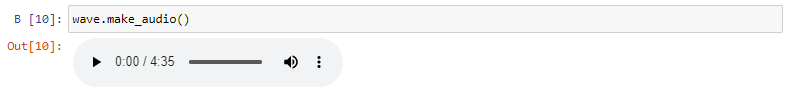
\includegraphics[width=\textwidth]{ex_4_wave_audio.png}
                \caption{Файл в аудио}
                \label{fig:ex_4_wave_audio}
            \end{figure}
            
            После этого получим спект из нашего сегмента:
            
\begin{lstlisting}[language=Python, caption= Получение спектра из сегмента]
    spectrum = segment.make_spectrum()
    spectrum.plot()
\end{lstlisting}   
            
             \begin{figure}[H]
                \centering
                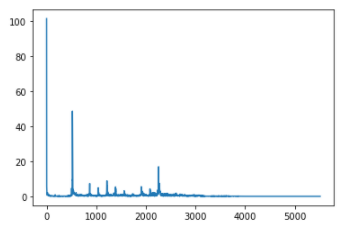
\includegraphics{ex_4_wave_spectr.png}
                \caption{Полученный спектр}
                \label{fig:ex_4_wave_spectr}
            \end{figure}
            
            И, наконец, полуим спектограмму для нашего сигнала:
            
\begin{lstlisting}[language=Python, caption= Получение спектограммы]
    wave.make_spectrogram(512).plot(high=5000)
    decorate(xlabel='Time (s)', ylabel='Frequency (Hz)')
\end{lstlisting}   
            
             \begin{figure}[H]
                \centering
                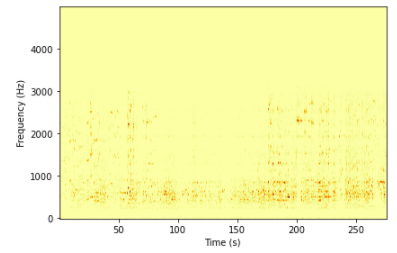
\includegraphics{ex_4_spectogramma.png}
                \caption{Полученная спектограмма}
                \label{fig:ex_4_spectogramma}
            \end{figure}
            
    
    \newpage
        \section{Часть №5: Создание \texttt{TromboneFliss}}
            В пятом пункте третьей лабораторной работы нам необходимо написать класс \texttt{TromboneFliss}, расширяюший \texttt{Chirp} и предоставляющий \texttt{evaluate}. Создать сигнал, имитирующий глиссандо на тромбоне от С3 до F3 и обратно.
            
            Для начала напишем класс \texttt{TromboneFliss}:
            
\begin{lstlisting}[language=Python, caption= Класс \texttt{TromboneFliss}]
    spectrum = segment.make_spectrum()
    spectrum.plot()
\end{lstlisting}   
            
            Теперь получим сигнал от 262 до 349 Гц и представим его в аудио формате:
            
            \begin{figure}[H]
                \centering
                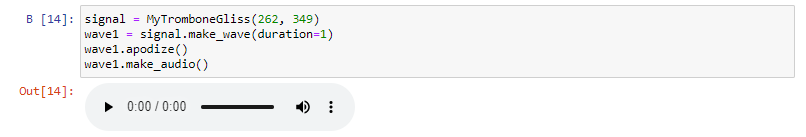
\includegraphics[width=\textwidth]{ex_5_signal_up_audio.png}
                \caption{Сигнал \texttt{up} в аудио}
                \label{fig:ex_5_signal_up_audio}
            \end{figure}
            
            После этого посмотрим на сегмент этого сигнала:
            
\begin{lstlisting}[language=Python, caption= Сегмент сигнала \texttt{up}]
    wave1.segment(start=0, duration=0.04).plot()
\end{lstlisting}   
            
             \begin{figure}[H]
                \centering
                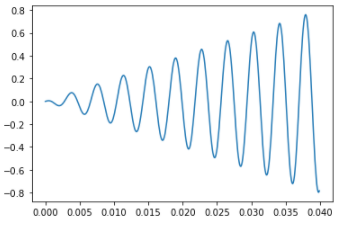
\includegraphics{ex_5_signal_up_segment.png}
                \caption{Полученный сегмент \texttt{up}}
                \label{fig:ex_5_signal_up_segment}
            \end{figure}
            
            Теперь получим обратный сигнал, от 349 до 262 Гц и так же представим его в виде оудио:
            
             \begin{figure}[H]
                \centering
                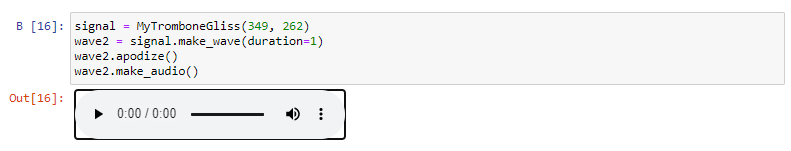
\includegraphics[width=\textwidth]{ex_5_signal_down_audio.png}
                \caption{Сигнал \texttt{down} в аудио}
                \label{fig:ex_5_signal_up_audio}
            \end{figure}
            
            И затем так же посмотрим на сегмент этого сигнала:
            
\begin{lstlisting}[language=Python, caption= Сегмент сигнала \texttt{down}]
    wave2.segment(start=0, duration=0.04).plot()
\end{lstlisting}   
            
             \begin{figure}[H]
                \centering
                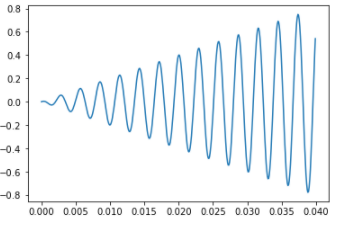
\includegraphics{ex_5_signal_down_segment.png}
                \caption{Полученный сегмент \texttt{down}}
                \label{fig:ex_5_signal_down_segment}
            \end{figure}
            
            После всего этого объедими эти два сигнала в один и получим аудиофайл:
            
            \begin{figure}[H]
                \centering
                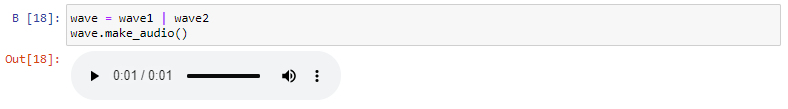
\includegraphics[width=\textwidth]{ex_5_signal_up_down_audio.png}
                \caption{Объединение \texttt{up} и \texttt{down} в аудио}
                \label{fig:ex_5_signal_up_down_audio}
            \end{figure}
            
            Затем получим спектр полученного сигнала:
            
\begin{lstlisting}[language=Python, caption= Спектр сигнала \texttt{up} и \texttt{down}]
    wave.make_spectrum().plot(high=500)
\end{lstlisting}   
            
             \begin{figure}[H]
                \centering
                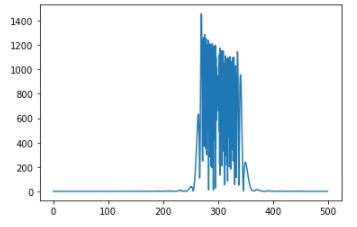
\includegraphics{ex_5_signal_up_down_spectr.png}
                \caption{Полученный спектр \texttt{up} и \texttt{down}}
                \label{fig:ex_5_signal_up_down_spectr}
            \end{figure}
            
            И, наконец, получим спектограмму полученного сигнала:
            
\begin{lstlisting}[language=Python, caption= Спектограмма сигнала \texttt{up} и \texttt{down}]
    wave.make_spectrogram(1024).plot(high=600)
    decorate(xlabel='Time (s)', ylabel='Frequency (Hz)')
\end{lstlisting}   
            
             \begin{figure}[H]
                \centering
                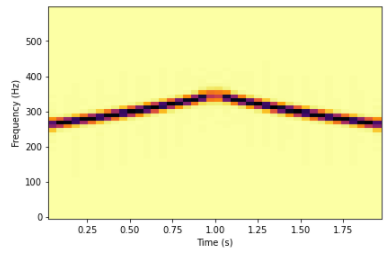
\includegraphics{ex_5_signal_up_down_spectogramma.png}
                \caption{Полученная спектограмма \texttt{up} и \texttt{down}}
                \label{fig:ex_5_signal_up_down_spectogramma}
            \end{figure}
           
    \newpage
        \section{Часть №6: Анализ букв}   
            В шестой части третьей лабораторной работы нам необходимо найти запись серии звуков букв алфавита. Необходимо построить спектограммы для этих звуков.
            
            В качестве аудиодорожки я взял запись с сайта FreeSounds, в которой проговариваются все буквы латинского алфавита, взял первый фрагмент с буквами a-e и после чего вывел данный сегмент:
            
\begin{lstlisting}[language=Python, caption= Вывод сегмента]
    wave = read_wave('67703__acclivity__alphabet-male.wav')
    segment = wave.segment(start=1, duration=7)
    segment.plot()
\end{lstlisting}   
            
             \begin{figure}[H]
                \centering
                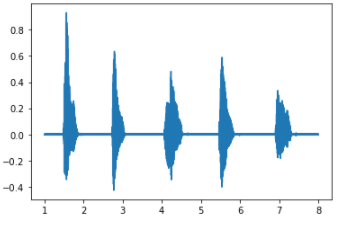
\includegraphics{ex_6_wave_segment.png}
                \caption{Полученный сегмент}
                \label{fig:ex_6_wave_segment}
            \end{figure}
            
            После этого проверим, что сигнал не поврежден, выведя его в видео аудио:
            
             \begin{figure}[H]
                \centering
                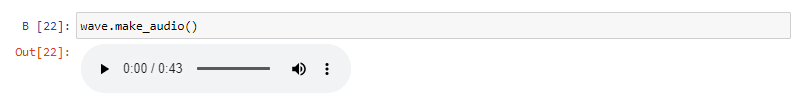
\includegraphics[width=\textwidth]{ex_6_wave_audio.png}
                \caption{Представление сигнала в аудио}
                \label{fig:ex_6_wave_audio}
            \end{figure}
            
            Затем получим спектограмму для нашего сегмента:
            
\begin{lstlisting}[language=Python, caption= Спектограмма для нашего сегмента]
    segment.make_spectrogram(1024).plot(high=1000)
    decorate(xlabel='Time (s)', ylabel='Frequency (Hz)')
\end{lstlisting}   
            
             \begin{figure}[H]
                \centering
                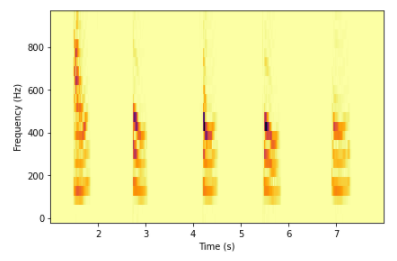
\includegraphics{ex_6_segment_spectogramma.png}
                \caption{Полученная спектограмма для сегмента}
                \label{fig:ex_6_segment_spectogramma}
            \end{figure}
            
            Теперь пройдемся по всем буквам из нашего сегмента, выводя сегменты на экран и представляя их в виде аудио. Начнем с первой буквы:
            
\begin{lstlisting}[language=Python, caption= Сегмент с буквой A]
    high = 1000
    segment = wave.segment(start=1, duration=1)
    segment.make_spectrum().plot(high=high)
    decorate(xlabel='Frequency (Hz)')
\end{lstlisting}   
            
             \begin{figure}[H]
                \centering
                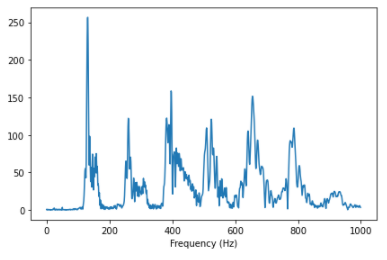
\includegraphics{ex_6_letter_a_segment.png}
                \caption{Сегмент с буквой A}
                \label{fig:ex_6_letter_a_segment}
            \end{figure}
            
            Представим сегмент с буквой A в виде аудиодорожки:
            
            \begin{figure}[H]
                \centering
                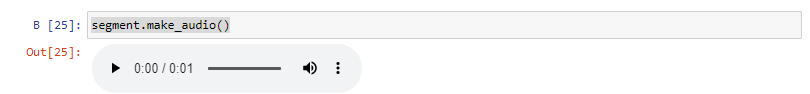
\includegraphics[width=\textwidth]{ex_6_letter_a_audio.png}
                \caption{Представление сегмента с буквой A в аудио}
                \label{fig:ex_6_letter_a_audio}
            \end{figure}
            
            Перейдем к сегменту с буквой В:
            
\begin{lstlisting}[language=Python, caption= Сегмент с буквой B]
    segment = wave.segment(start=2, duration=1)
    segment.make_spectrum().plot(high=high)
    decorate(xlabel='Frequency (Hz)')
\end{lstlisting}   
            
             \begin{figure}[H]
                \centering
                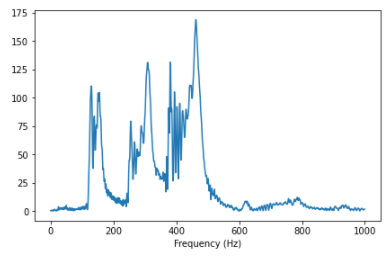
\includegraphics{ex_6_letter_b_segment.png}
                \caption{Сегмент с буквой B}
                \label{fig:ex_6_letter_b_segment}
            \end{figure}
            
            Представим сегмент с буквой B в виде аудиодорожки:
            
            \begin{figure}[H]
                \centering
                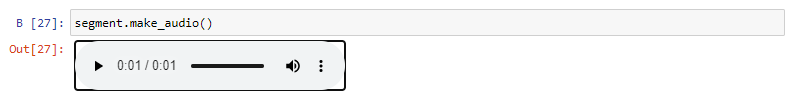
\includegraphics[width=\textwidth]{ex_6_letter_b_audio.png}
                \caption{Представление сегмента с буквой B в аудио}
                \label{fig:ex_6_letter_b_audio}
            \end{figure}
            
             Перейдем к сегменту с буквой C:
            
\begin{lstlisting}[language=Python, caption= Сегмент с буквой C]
    segment = wave.segment(start=3.5, duration=1)
    segment.make_spectrum().plot(high=high)
    decorate(xlabel='Frequency (Hz)')
\end{lstlisting}   
            
             \begin{figure}[H]
                \centering
                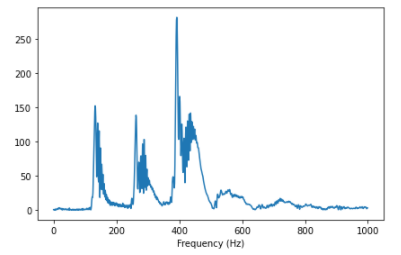
\includegraphics{ex_6_letter_c_segment.png}
                \caption{Сегмент с буквой C}
                \label{fig:ex_6_letter_c_segment}
            \end{figure}
            
            Представим сегмент с буквой C в виде аудиодорожки:
            
            \begin{figure}[H]
                \centering
                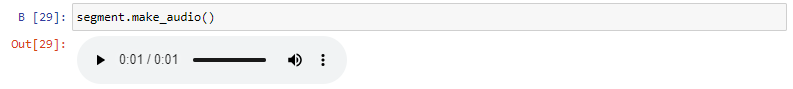
\includegraphics[width=\textwidth]{ex_6_letter_c_audio.png}
                \caption{Представление сегмента с буквой C в аудио}
                \label{fig:ex_6_letter_c_audio}
            \end{figure}
            
             Перейдем к сегменту с буквой D:
            
\begin{lstlisting}[language=Python, caption= Сегмент с буквой D]
    segment = wave.segment(start=5, duration=1)
    segment.make_spectrum().plot(high=high)
    decorate(xlabel='Frequency (Hz)')
\end{lstlisting}   
            
             \begin{figure}[H]
                \centering
                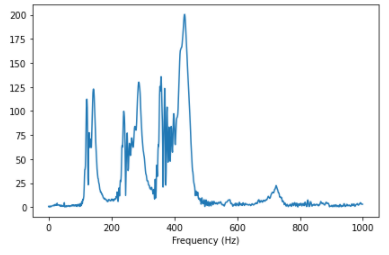
\includegraphics{ex_6_letter_d_segment.png}
                \caption{Сегмент с буквой D}
                \label{fig:ex_6_letter_d_segment}
            \end{figure}
            
            Представим сегмент с буквой D в виде аудиодорожки:
            
            \begin{figure}[H]
                \centering
                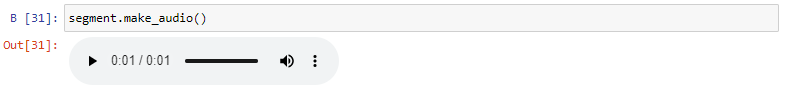
\includegraphics[width=\textwidth]{ex_6_letter_d_audio.png}
                \caption{Представление сегмента с буквой D в аудио}
                \label{fig:ex_6_letter_d_audio}
            \end{figure}
            
             Перейдем к сегменту с буквой E:
            
\begin{lstlisting}[language=Python, caption= Сегмент с буквой E]
    segment = wave.segment(start=6.5, duration=1)
    segment.make_spectrum().plot(high=high)
    decorate(xlabel='Frequency (Hz)')
\end{lstlisting}   
            
             \begin{figure}[H]
                \centering
                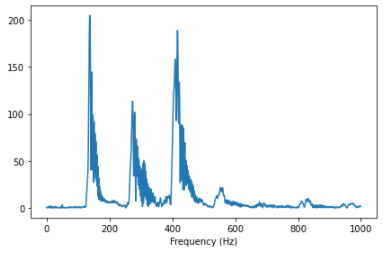
\includegraphics{ex_6_letter_e_segment.png}
                \caption{Сегмент с буквой E}
                \label{fig:ex_6_letter_e_segment}
            \end{figure}
            
            Представим сегмент с буквой E в виде аудиодорожки:
            
            \begin{figure}[H]
                \centering
                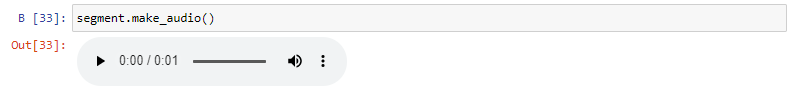
\includegraphics[width=\textwidth]{ex_6_letter_e_audio.png}
                \caption{Представление сегмента с буквой E в аудио}
                \label{fig:ex_6_letter_e_audio}
            \end{figure}
            
            В результате выполнения данного пункта можно сделать вывод о том, что гласные звуки при представлении их в виде сегмента имеют более выраженный пик и большую частоту, чем согласные звуки. 
            
    \newpage
        \section{Выводы}
             В результате выполнения данной лабораторной работы мы изучили как надо работать с апериодическими сигналами, что такое чирп, каков его спектр. Также научились строить спектограммы чирпов, работать с утечкаи. Кроме того были реализованы и проверены классы для реализации чирпа, и для создания имитации глиссандо на тромбоне. 
           
\end{document}
